\documentclass{amsart}
\usepackage{graphicx, amsthm}
\usepackage{float}
\usepackage{enumerate}
\restylefloat{figure} 
\usepackage{tikz} 
\newcommand{\Z}{\mathbb{Z}}
\newcommand{\N}{\mathbb{N}}
\newcommand{\R}{\mathbb{R}}
\usepackage{hyperref}
\newcommand{\e}{\mathbf{e}}

\theoremstyle{definition} \newtheorem*{definition}{Definition} 
\theoremstyle{remark} \newtheorem*{ex}{Example} 


\title{Exercise set $5$, \\ MS-A0402, Foundations of Discrete Mathematics}
\begin{document}
\hspace{-1cm}
\maketitle
 
\section*{Explorative exercises}
I recommend that you study the explorative problems before the first lecture of the week.\\

A {\em graph} $G=(V,E)$ is a set of {\em nodes} (or vertices) $V$ together with a set $E$ of {\em edges}, each of which connects two nodes with each other. Two graphs $G=(V,E)$ and $G'=(V,E')$ are said to be {\em isomorphic} if there is a bijection $\phi:V\to V'$ such that there is an edge between $u$ and $v$ in $G$ if and only if there is an edge between $\phi(u)$ and $\phi(v)$ in $G'$. Intuitively, this means that the graphs $G$ and $G'$ are ``the same'', and $\phi(u)$ tells what node in $G'$ is ``the same'' as the node $u\in G$. 

\subsection*{Problem 1}To check that you have understood the definition, convince yourself that the graphs below are isomorphic!
\begin{center}
\includegraphics[width=3cm]{4cyc1}\hspace{1cm}\includegraphics[width=3cm]{4cyc2}
\end{center}


\subsection*{Problem 2} The following figure shows three graphs with six vertices. Are they isomorphic?
\begin{center}
\includegraphics[width=9cm]{graphs2}
\end{center}

 \subsection*{Problem 3}
A tree is a graph that is connected and has no cycles. (Ask if you do not understand these terms.) 
\begin{enumerate}[a)]
\item Show that a tree with $n$ nodes always have exactly $n-1$ edges. 
\item Convince yourself that all trees with three nodes are isomorphic.
\item Draw as many non-isomorphic trees with four nodes as you can. Can you prove that there are not any more?
\item Draw as many non-isomorphic trees with five nodes as you can. Can you prove that there are not any more?
\item Draw as many non-isomorphic trees with six nodes as you can. Can you prove that there are not any more?
\end{enumerate}

\pagebreak

 \section*{Homework}
The written solutions to the homework problems should be handed in on MyCourses by Monday 4.4., 12:00. You are allowed and encouraged to discuss the exercises with your fellow students, but everyone should write down their own solutions.

\subsection*{Problem 1}(10pts)
Consider the permutations $$\rho=\begin{pmatrix}1&2&3&4&5\\3&1&2&5&4\end{pmatrix}\mbox{ and }\sigma=\begin{pmatrix}1&2&3&4&5\\1&5&2&3&4\end{pmatrix}.$$ Are they conjugates? If so, find a permutation $\tau$ such that $\tau\rho\tau^{-1}=\sigma$.

\subsection*{Problem 2}(10pts)
The \textbf{perfect riffle shuffle} (or ``\textit{Faro shuffle}'') of a deck consisting of $2n$ cards (for a fixed $n \in \N$) is a permutation 
$$\sigma = \begin{pmatrix}1&2&3&4&\dots&  2n-1 & 2n \\1&n+1&2&n+2&\dots & n & 2n\end{pmatrix} \in S_{2n}$$
that splits a deck of $2n$ cards into two piles and interleaves them (i.e. card in position 1 goes to position 1, card in position 2 goes to position $n+1$, card in position 3 goes to position 3, card in position 4 goes to position $n+2$, etc.).  This is also called an out-shuffle, because it leaves the top card at the top and bottom card at the bottom. Thus we can write a formula:
$$\sigma(k) = \begin{cases}
\frac{k+1}{2}, & k \text{ is odd}\\
n+\frac{k}{2}, & k \text{ is even}\\
\end{cases}$$
Let $n = 3$, that is, we have a deck of $6$ cards. Find the number of perfect riffle shuffles needed to return the deck to its original state. In order words, find some $N \in \N$ such that 
$$\sigma^N = \underbrace{\sigma \sigma \sigma \dots \sigma \sigma}_{N \text{ times}} =  e,$$
where $e \in S_{2n}$ is the identity permutation $e(i) = i$ for all $i \in \{1,2,\dots,2n\}$. 

\textit{Hint: for a deck of 52 cards, that is, when $n = 26$, this can be done with $8$ shuffles, that is, $\sigma^8 = e$ ( proof: \url{https://www.youtube.com/watch?v=7lNk7bfkFq8} ), so it probably is less than $8$ here with just 6 cards.}

\subsection*{Problem 3} (10pts) The following figure shows two graphs with eleven vertices. The graph on the left has $V=\{0,1,2,\dots, 10\}$, whereas the one on the right has nodes $V'=\{a,b,\dots, k\}$. Are they isomorphic?
\begin{center}
\includegraphics[width=8cm]{graphs}
\end{center}

\subsection*{Problem 4} (10pts) Colour the following graph with the greedy algorithm.
\begin{center}
\includegraphics[width=3cm]{petersen}
\end{center}
Can you find an ordering of the vertices such that the greedy algorithm colours the graph with $3$ colors?





\section*{Additional problems}

These do not need to be returned for marking.

\subsection*{Problem 1}
A farmer needs to carry a wolf, a goat, and a cabbage across a river. The farmer only has a small boat, which can carry the farmer and only one object (an animal or a vegetable). He can cross the river repeatedly. However, the wolf must not be left alone with the goat, and the goat must not be left alone with the cabbage.

We can describe each state (when the farmer is on one of the shores with the boat) by listing what is on each shore. For example, the pair $(FG,WC)$ represents the state where the farmer and goat (and the boat) are on the first shore and the wolf and cabbage are
on the other shore.

\begin{enumerate}[a)]
\item Find all allowed states of the puzzle.
\item Draw a graph whose vertices
are the allowed states, that has an edge connecting two states between which the farmer can go using the boat once.
\item Explain why finding a path from the vertex $(FWGC,\emptyset)$ to the vertex  $(\emptyset, FWGC)$
solves the puzzle.
\item Find two different solutions of the puzzle, each using
seven crossings.
\end{enumerate}


\subsection*{Problem 2}
The {\em dihedral group} $D_4$ consists of those permutations $\sigma\in S_4$ that are isomorphisms of the graph $C_4$.
For example $\sigma=(12)\not\in D_4$, because there is an edge between the nodes $2$ and $3$, but not between the nodes $\sigma(2)=1$ and $\sigma(3)=3$.
\begin{center}
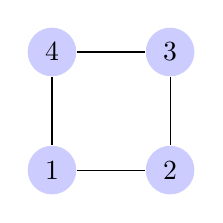
\begin{tikzpicture}
  [scale=.5,auto=left,every node/.style={circle,fill=blue!20}]
  \node (n1) at (0,0) {1};
  \node (n2) at (3,0)  {2};
  \node (n3) at (3,3)  {3};
  \node (n4) at (0,3)  {4};

  \foreach \from in{n1, n3}
  \foreach \to in{n2, n4}
    \draw (\from) -- (\to);
\end{tikzpicture}
\end{center}
\begin{enumerate}[a)]  
\item  How many permutations are there in $D_4$?
\item Prove that all permutations in $D_4$ can be written as a product of the rotation $\rho=(1234)$ and the reflection $\pi=(13)$.
\end{enumerate}

\subsection*{Problem 3}
Find the shortest path from the node $a$ to the node $z$ in the graph below.
\begin{center}
\includegraphics[width=5cm]{shortestpath}
\end{center}

\subsection*{Problem 4}
For a graph $G$, we denote its chromatic number $\chi(G)$, the size of its largest clique $\omega(G)$, and the maximum degree $\Delta(G)$. Find an exampe of a graph $G$ such that $$\omega(G)<\chi(G)<\Delta(G).$$ 

\subsection*{Problem 5}
Compute (with proof) the chromatic number of the Gr\"otszch graph, depicted below. [2p]
\begin{center}
\includegraphics[width=1.5cm]{grotszch}
\end{center}

\subsection*{Problem 6}
Professor X and her husband Mr X are inviting four other couples to a dinner party. In the beginning of the party, some of the participants shake hands with each other. However, nobody shakes hands with their own spouse (or with themselves). In the end of the party, Professor X asks all other participants how many people they shook hands with, and gets nine different answers. How many guests did Mr X shake hands with?

\subsection*{Problem 7}
Is the following statement true or false? ``At every party, there are at least two people who know the same number of other guests.''
\begin{enumerate}[a)]
 \item If the relation ``A knows B'' is assumed to be symmetric. (If I know (am friends with) Bob, then Bob knows (is friends with) me.)
\item If the relation ``A knows B'' is {\em not} assumed to be symmetric. (I know (have heard about) Bob Dylan, but Bob Dylan doesn't know (hasn't heard about) me.)
\end{enumerate}


\end{document}  